\documentclass[a4paper,10pt]{scrreprt}
%\documentclass[a4paper,10pt]{scrartcl}

\usepackage[utf8]{inputenc}
\usepackage[german]{babel}
\usepackage[pdftex]{graphicx}
\usepackage{listings}
\usepackage{color}
\usepackage{amssymb}
\usepackage{marvosym}
\usepackage{amsmath}
\usepackage{array}
\usepackage{geometry}
\usepackage{color}

\newcommand{\f}{\noindent\textbf}
\geometry{verbose,tmargin=2cm,bmargin=2.5cm,lmargin=2.5cm,rmargin=3cm,headheight=80pt}

\title{FIA - WS 2014/15}
\author{}
\date{}

\begin{document}
\maketitle

\chapter{Introduction}
\section{Internet}

\begin{itemize}
 \item loosely hierarchical: tier 1 to tier 3
 \item communications infrastructure enables distributed applications
 \item hyper... $\Rightarrow$ concentration of content (Amazon, Google, ...)
\end{itemize}

\section{Protocol Layering}
\begin{itemize}
 \item ISO/OSI
 \item TCP, UDP, ICMP, UDP Like, SCTP, ...
 \item DHCP, NAT, ...
\end{itemize}

\section{Analogue digital conversion}
\begin{itemize}
 \item Fourier transformation 
 \item sampling theorem + Nyquist
 \item PCM-transmission 
 \item small amplitudes are being encoded more detailed than large amplitudes
\end{itemize}

\section{Color Coding}
\begin{itemize}
 \item monochrome, RGB, YCbCr
 \item RGB: 
 \begin{itemize}
  \item red, green, blue values between [0,  \{7,31,...,65535\}]
  \item nonlinear encoding of intensities 
  \item computer graphics
 \end{itemize}
 \item YCbCr
 \begin{itemize}
  \item TV and digital video
  \item Y more important $\Rightarrow$ encode with more details 
  \item more efficient than RGB
  \item can handle downsampling better
  \item YUV is based color model used in analog color TV
  \begin{itemize}
   \item YCbCr is scaled and offset version
   \item YPbPr is the analog version of YCbCr
  \end{itemize}
 \end{itemize}
\end{itemize}

\chapter{Digital coding of audio and video}
\section{Rate-Distortion Theory}
\begin{itemize}
 \item lossless compression algorithms 
 \begin{itemize}
  \item allow perfect reconstruction 
  \item low compression ratios
  \item frequently encountered data is encoded more efficiently 
 \end{itemize}
 \item lossy compression algorithms
 \begin{itemize}
  \item result is only a close approximation of original data
  \item trade-off: distortion vs. required rate 
  \item much higher compression rate than lossless compression
 \end{itemize}
//TODO: bild einfuegen
 \item rate and distortion as measures for efficiency of compression and difference between reconstructed and original data 
 \begin{itemize}
  \item goal is to minimize distortion and rate 
  \item basic problem:
  \begin{itemize}
   \item minimum expected distortion at a given rate?
   \item minimum rate to achieve given distortion?  
  \end{itemize}
 \end{itemize}
 \item distortion measures
 \begin{itemize}
  \item mean square error $\sigma^2 = \frac{1}{N}\sum\limits_{i=1}^N(x_i - y_i)^2$
  \item signal to noise ratio $SNR = 10 log_{10}\frac{\sigma_x^2}{\sigma_d^2}$
  \item peak signal to noise ratio $PSNR = 10 log_{10}\frac{x_{peak}^2}{x_d^2}$
 \end{itemize}
 \item in order to maximize efficient communication maximize mutual information between x and y 
 \item rate distortion function 
\end{itemize}

\section{digital image}
\begin{itemize}
 \item conversion between RGB and YUV
 \item downsampling J:a:b
 \begin{itemize}
  \item 4:4:4 $\widehat{=}$ no downsampling
  \item 4:2:2 $\widehat{=}$ 
  \item 4:2:0 $\widehat{=}$ 
 \end{itemize}
 \item statistical image modeling 
 \begin{itemize}
  \item all natural images occupy a tiny and unknown sloped space of all images 
  \item pixel intensities are dependent and correlated to the corresponding image $\Rightarrow$ pixel within images are highly correlated 
  \item correlation of pixels has high impact on image compression
 \end{itemize}
 \item image transformations 
 \begin{itemize}
  \item negative transformations
  \item log transformations
  \item power-law transformations
 \end{itemize}
 \item intensity:
 \begin{itemize}
  \item change in brightness $\Rightarrow$ shift of histogram
  \item change in contrast $\Rightarrow$ stretch/? of histogram
 \end{itemize}
\item filters based on convolution of neighbor pixels $\Rightarrow$ enhancement, smoothing, edge, detection, ...
\item the hoar transform 
\begin{itemize}
 \item simplest useful energy compression
 \item lossless retransformation is possible 
 \item transform original image into 4 parts (in 20)
 \begin{enumerate}
  \item top-left: a+b+c+d, 4 point average, very important
  \item top-right: a-b+c-d, average horizontal gradient, less important
  \item bottom-left: a+b-c-d, average vertical gradient, less important
  \item bottom-right: a-b-c+d, diagonal curvature, less important
 \end{enumerate}
 \item 1 is more expensive while 2-4 is cheaper to encode 
 \item reordering required to provide ``typical'' representation
\end{itemize}
 \item entropy -- quantifying the required bitrate
 \begin{itemize}
  \item entropy $H_x$ represents the mean number of bits per pixel that are required to encode the image 
  \item $H_x = \sum\limits_{i=0}^{M-1} p_i-log_2\left(\frac{1}{p_i}\right)$ where $p_i = \frac{\text{pixel in bin i}}{N}$ where N is the number of pixels
  \item estimated number of bits needed is $H_x\cdot N$
 \end{itemize}
 \item the Karkunen-Loeve transform (KLT)
 \begin{itemize}
  \item is optimal for minimizing bitrate
  \item not or seldom used in practice $\Rightarrow$ slow and complex
 \end{itemize}
 \item the discrete cosine transformation (DCT)
 \begin{itemize}
  \item seems to put most energy on a small number of values
  \item linear transformation
  \item each real world image can be represented by a combination of the DCT bases
  \item DCT bases fit better to typical images than FFT or DST
  \item first coefficient of DCT is mean of values being transformed and represents average tone of the block. subsequent blocks add further detail
  \item JPEG: $8\times 8$ DCT (empirically found to be good)
 \end{itemize}
 \item need for wavelets
 \begin{itemize}
  \item signals are available in time-domain but processing frequency information is much more easy
  \item transformations (e.g. FFT) translate time-domain signals into frequency domains
  \begin{itemize}
   \item useful for stationary signals where all frequencies are present at all times
   \item not useful for instationary signals: both information required
   \item solution: short term transformation---transformation of small fixed timewindows (similar to blocks of images)
  \end{itemize}
  \item wavelet analysis uses different sized windows
  \begin{itemize}
   \item high frequency parts $\Rightarrow$ small windows $\Rightarrow$ good time resolution
   \item low frequency parts $\Rightarrow$ big windows $\Rightarrow$ good frequency resolution
  \end{itemize}
 \end{itemize}
\end{itemize}
\section{JPEG compression}
\begin{itemize}
 \item joint photographic experts groups
 \item 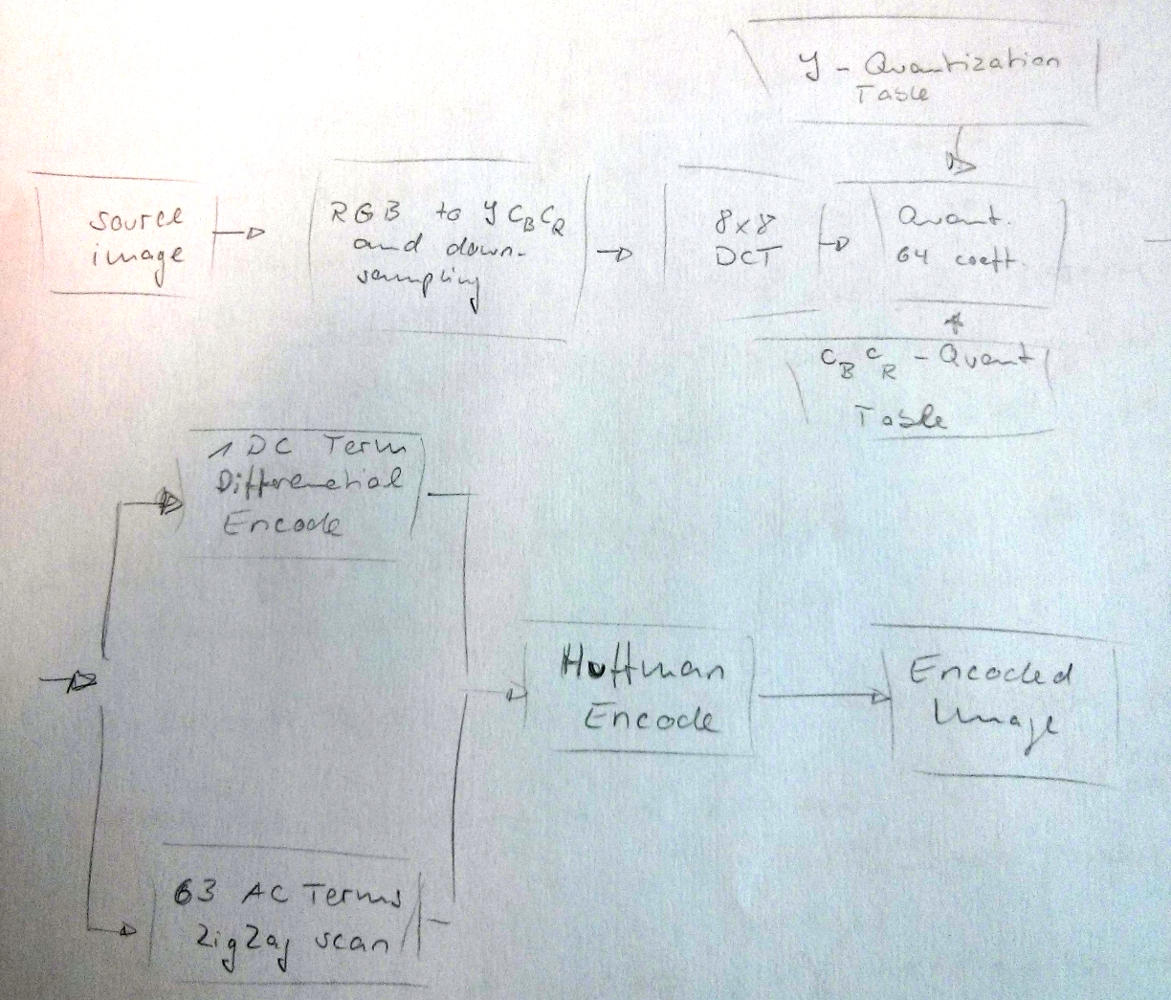
\includegraphics[width=.8\linewidth]{jpeg.jpg}
\end{itemize}
\section{digital video}
\begin{itemize}
 \item high corellation between successive frames
 \item interframe differential pulse code modulation ($\Rightarrow$ vgl. skript skizze)
 \item frame replenishment $\Rightarrow$ pixels are only transmitted if a specified threshold is exceeded, otherwise nothing is transmitted
 \item change detection
 \begin{itemize}
  \item pixel wise change detector
  \item block wise change detector
  \item comparision between current and previous frame
  \begin{itemize}
   \item substract previous frame from current one
   \item convert to absolute value
   \item generate $3\times 3$ averages
   \item check for threshold
  \end{itemize}
 \end{itemize}
 \item motion compensated coding 
 \begin{itemize}
  \item changes between frames due to moving objects $\Rightarrow$ estimation of motion vectors
  \item prediction and original frame may differ significantly
  \begin{itemize}
   \item solution: compute and transmit prediction error additionally
   \item higher coding efficiency but also higher computational complexity
  \end{itemize}
  \item three-stage-coding:
  \[ \text{Motion Analysis} \Rightarrow \text{Prediction and differentiation} \Rightarrow \text{Encoding} \]
 \end{itemize}
 \item block matching
 \begin{itemize}
  \item partitioning of frame into nonoverlapping equally spaced and fixed size rectangular blocks
  \item smaller block size $\Rightarrow$ better approximation but higher computational complexity
  \item $16 \times 16 $ blocks used in MPEG-1 and -2
  \item calculate best displacement vector for each block
  \item search strategies:
  \begin{itemize}
   \item full search
   \item 2D logarithmic search
   \item diamond search
  \end{itemize}
  \item grouping of elements
  \begin{itemize}
   \item 
  \end{itemize}


 \end{itemize}


\end{itemize}



\end{document}
